% -*- latex -*-
%%%%%%%%%%%%%%%%%%%%%%%%%%%%%%%%%%%%%%%%%%%%%%%%%%%%%%%%%%%%%%%%
%%%%%%%%%%%%%%%%%%%%%%%%%%%%%%%%%%%%%%%%%%%%%%%%%%%%%%%%%%%%%%%%
%%%%
%%%% This text file is part of the source of 
%%%% `Parallel Programming in MPI and OpenMP'
%%%% by Victor Eijkhout, copyright 2012-2022
%%%%
%%%% mpi-onesided.tex : about onesided communication
%%%%
%%%%%%%%%%%%%%%%%%%%%%%%%%%%%%%%%%%%%%%%%%%%%%%%%%%%%%%%%%%%%%%%
%%%%%%%%%%%%%%%%%%%%%%%%%%%%%%%%%%%%%%%%%%%%%%%%%%%%%%%%%%%%%%%%

\index{communication!one-sided|(}
\index{target!active synchronization|see{active target synchronization}}
\index{target!passive synchronization|see{passive target synchronization}}

Above, you saw  point-to-point operations of the two-sided type:
they require the co-operation of a sender and
receiver. This co-operation could be loose: you can post a receive
with \indexmpishow{MPI_ANY_SOURCE} as sender, but there had to be both a send and
receive call. This two-sidedness can be limiting. Consider code where the receiving
process is a dynamic function of the data:
\begin{lstlisting}
x = f();
p = hash(x);
MPI_Send( x, /* to: */ p );
\end{lstlisting}
The problem is now: how does \lstinline{p} know to post a receive,
and how does everyone else know not to?

In this section, you will see one-sided communication 
routines where a process
can do a `put' or `get' operation, writing data to or reading it from
another processor, without that other processor's involvement.

In one-sided MPI operations, 
known as \acf{RMA} operations in the standard,
or as \acf{RDMA} in other literature,
there
are still two processes involved: the \indexterm{origin}, which is the
process that originates the transfer, whether this is a `put' or a `get',
and the \indexterm{target} whose
memory is being accessed. Unlike with two-sided operations, the target
does not perform an action that is the counterpart of the action on the origin.

That does not mean that the origin can access arbitrary data on the target
at arbitrary times. First of all, one-sided communication in MPI
is limited to accessing only a specifically declared memory area on the target:
the target declares an area of
memory that is accessible to other processes. This is known
as a \indexterm{window}. Windows limit how origin processes can access
the target's memory: you can only `get' data from a window or `put' it
into a window; all the other memory is not reachable from other processes.
On the origin there is no such limitation;
any data can function as the source of a `put'
or the recipient of a `get operation.

The alternative to having windows is to use \indexterm{distributed shared memory}
or \indexterm{virtual shared memory}: memory is distributed but acts as if
it shared. The so-called \acf{PGAS} languages such as \ac{UPC} use this model.

Within one-sided communication, MPI has two modes: active RMA and
passive RMA. In \indextermsub{active}{RMA}, or \indexterm{active target synchronization},
the target sets boundaries on the time period (the `epoch')
during which its window can be accessed.
The main advantage
of this mode is that the origin program can perform many small transfers, which are
aggregated behind the scenes.
This would be appropriate for applications that are structured
in a \ac{BSP} mode with \indexterm{superstep}s.
Active RMA acts much like asynchronous transfer with a
concluding \indexmpishow{MPI_Waitall}.

In \indextermsub{passive}{RMA}, or \indexterm{passive target synchronization},
the target process puts no limitation on when its window can be accessed.
(\ac{PGAS} languages such as \ac{UPC} are based on this model: data is 
simply read or written at will.)
While 
intuitively it is attractive to be able to write to and read from a target at
arbitrary time,
there are problems. For instance, it requires a remote agent on the target,
which may interfere with execution of the main thread, or conversely it may not be
activated at the optimal time. Passive RMA is also very hard to debug and can lead
to race conditions.

%% McLaren says use an info object

\Level 0 {Windows}
\label{sec:windows}
\index{window|(}

\begin{figure}[ht]
  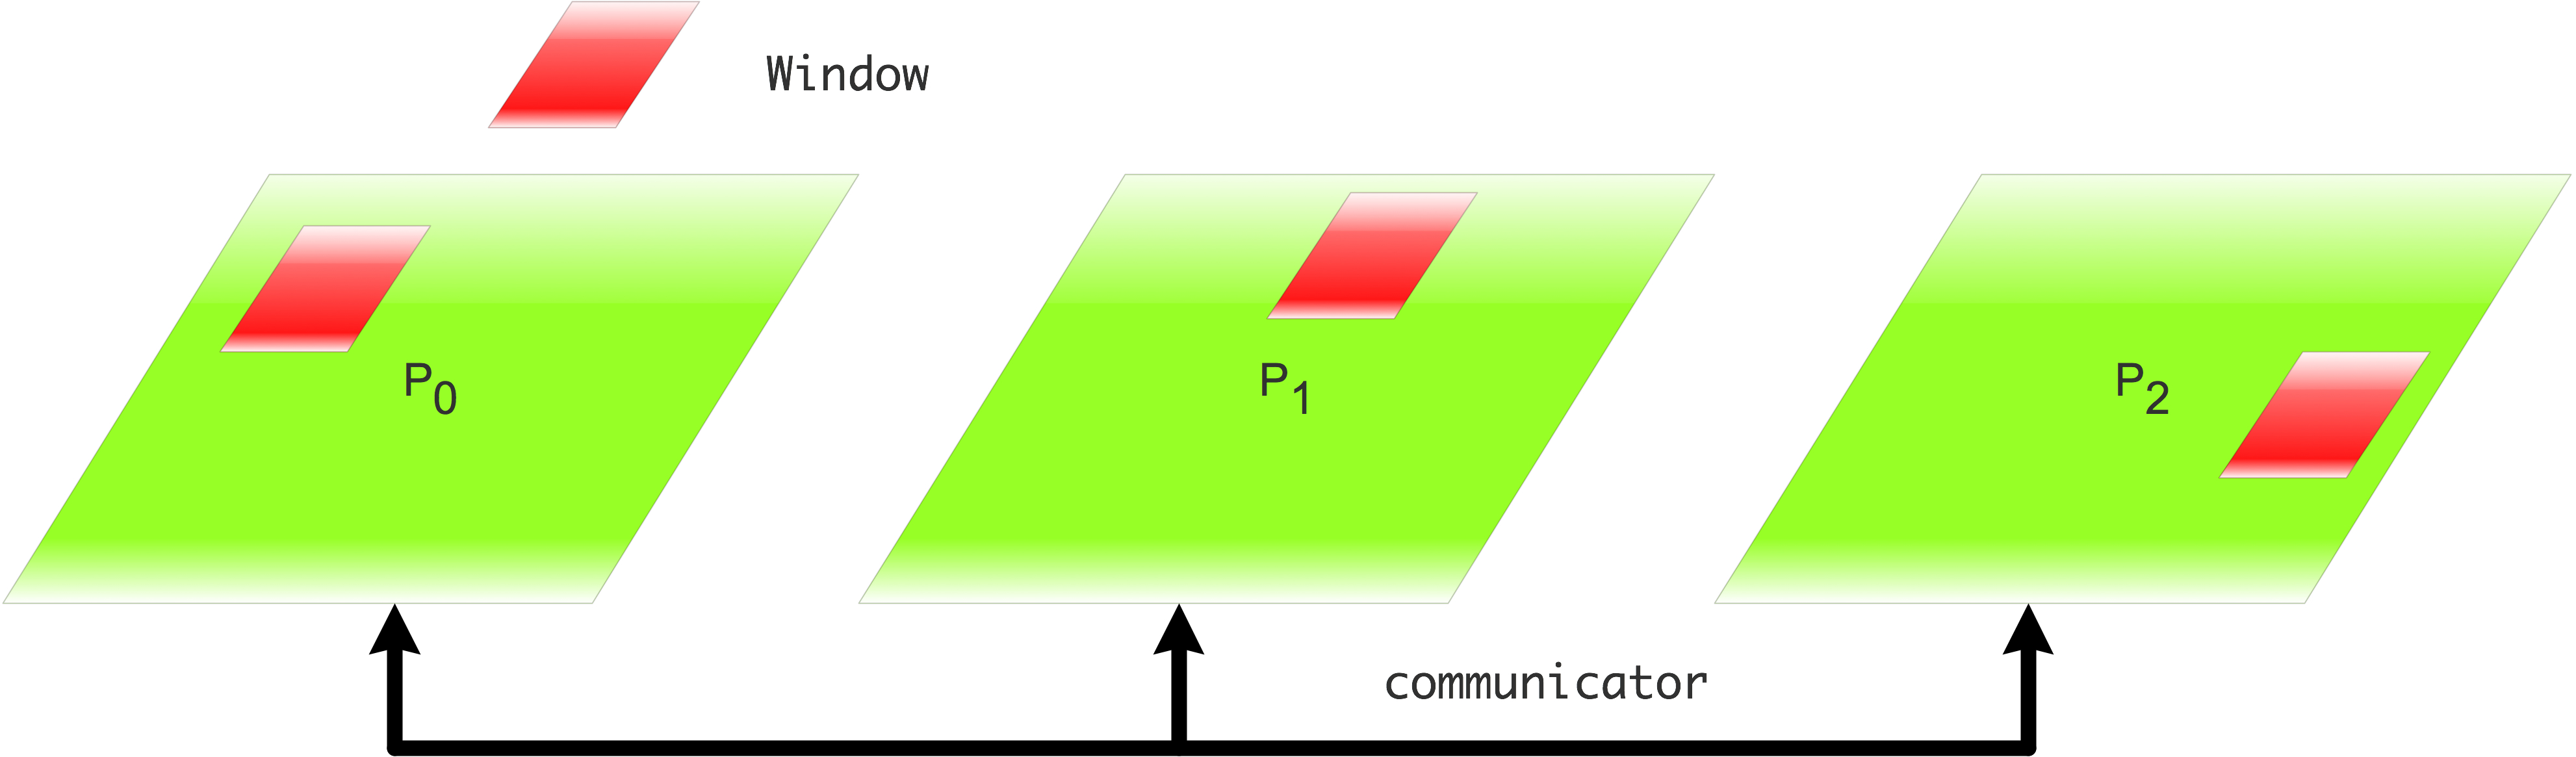
\includegraphics[scale=.1]{one-sided-window}
  \caption{Collective definition of a window for one-sided data access}
  \label{fig:window}
\end{figure}

In one-sided communication, each processor can make an area of memory,
called a \indexterm{window}, available to one-sided transfers.
%
This is stored in a variable of type \indexmpidef{MPI_Win}.
%
A~process can put an arbitrary item from its own memory
(not limited to any window) to the window of another process,
or get something from the other process'
window in its own memory.

A window can be characteristized as follows:
\begin{itemize}
\item The window is defined on a communicator, so the create call
  is collective; see figure~\ref{fig:window}. 
\item The window size can be set individually on each process.
  A~zero size is allowed, but since window creation is collective,
  it is not possible to skip the create call.
\item You can set a `displacement unit' for the window: this is a number of
  bytes that will be used as the indexing unit. For example if you use
  \lstinline{sizeof(double)} as the displacement unit,
  an~\lstinline{MPI_Put} to location~8 will go to the 8th double.
  That's easier than having to specify the 64th byte.
\item The window is the target of data in a put operation, or the
  source of data in a get operation; see figure~\ref{fig:putget}.
\item There can be memory associated with a window, so it needs to be
  freed explicitly with \indexmpishow{MPI_Win_free}.
\end{itemize}

The typical calls involved are:
\lstset{style=reviewcode,language=C}
\begin{lstlisting}
MPI_Info info;
MPI_Win window;
MPI_Win_allocate( /* size info */, info, comm, &memory, &window );
// do put and get calls
MPI_Win_free( &window );
\end{lstlisting}

\begin{figure}[ht]
  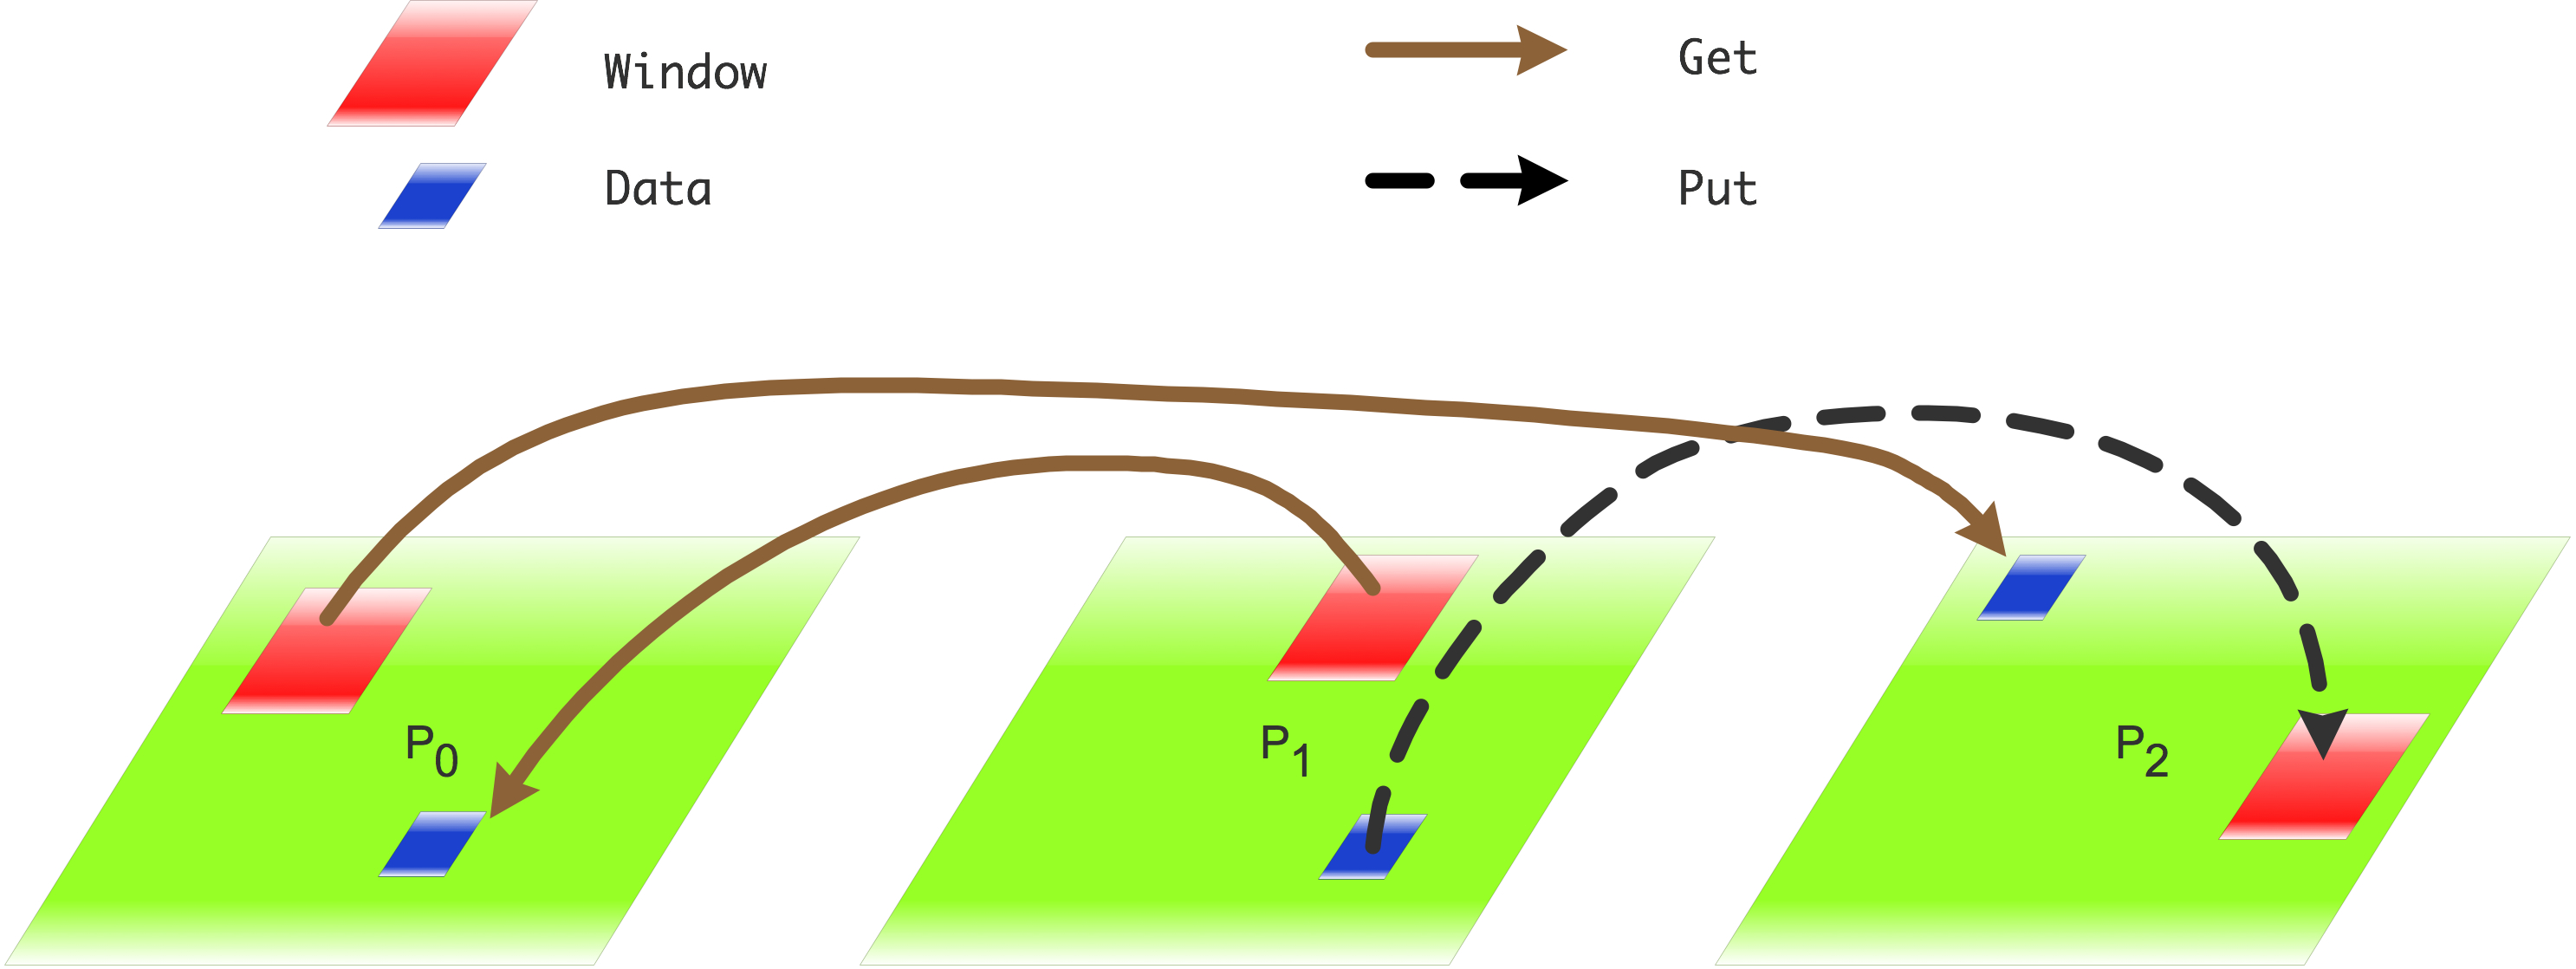
\includegraphics[scale=.1]{one-sided-getput}
  \caption{Put and get between process memory and windows}
  \label{fig:putget}
\end{figure}

\Level 1 {Window creation and freeing}
\label{sec:win-alloc}
\index{window!memory allocation|(}

The memory for a window is at first sight ordinary data in user space. There are multiple
ways you can associate data with a window:
\begin{enumerate}
\item You can pass a user buffer to
  \indexmpiref{MPI_Win_create}. This buffer can be an ordinary array,
  or it can be created with \indexmpishow{MPI_Alloc_mem}.
  (In the former case, it may not be possible to lock the window;
  section~\ref{sec:passive-sync}.)
\item You can let MPI do the allocation, so that MPI can perform various
  optimizations regarding placement of the memory. The user code then
  receives the pointer to the data from MPI. This can again be done in two ways:
  \begin{itemize}
  \item Use \indexmpiref{MPI_Win_allocate} to create the data and the
    window in one call.
  \item If a communicator is on a shared memory (see
    section~\ref{mpi-comm-split-type}) you can create a window in that
    shared memory with \indexmpishow{MPI_Win_allocate_shared}.
    This will be useful for
    MPI \emph{shared memory}\index{memory!shared, MPI};
    see chapter~\ref{ch:mpi-shared}.
  \end{itemize}
\item Finally, you can create a window with
  \indexmpishow{MPI_Win_create_dynamic} which postpones the allocation;
  see section~\ref{sec:win-dynamic}.
\end{enumerate}

First of all, \indexmpishow{MPI_Win_create}
creates a window from a pointer to memory.
The data array must not be \n{PARAMETER} or \n{static const}.

The size parameter is measured in bytes. In~C this can be done
with the \indextermtt{sizeof} operator;
%
\cverbatimsnippet[examples/mpi/c/examples/putfencealloc.c]{windowsizeof}
%
for doing this calculation in Fortran, see section~\ref{sec:mpif-shape}.

\begin{pythonnote}{Displacement byte computations}
  For computing the displacement in bytes,
  here is a good way for finding the size of \indexterm{numpy} datatypes:
  \pverbatimsnippet[examples/mpi/p/putfence.py]{windispp}
\end{pythonnote}

Next, one can obtain the memory from MPI by using
\indexmpirep{MPI_Win_allocate},
which has the data pointer as output. Note the \n{void*} in the
C~signature; it is still necessary to pass a pointer to a pointer:
\begin{lstlisting}
double *window_data;
MPI_Win_allocate( ... &window_data ... );
\end{lstlisting}
The routine \indexmpiref{MPI_Alloc_mem} performs only the allocation
part of \indexmpishow{MPI_Win_allocate}, after which you need to
\indexmpishow{MPI_Win_create}.
\begin{itemize}
\item
  An error of \indexmpishow{MPI_ERR_NO_MEM} indicates that
  no memory could be allocated.
\begin{mpifournote}{Info key for alignment}
  \item 
    Allocated memory can be aligned by specifying an \indexmpishow{MPI_Info} key
    of \indexmpishow{mpi_minimum_memory_alignment}.
\end{mpifournote}
\end{itemize}

This memory is freed with \indexmpidef{MPI_Free_mem}:
\cverbatimsnippet{winallocate}
(Note the lack of an ampersand in the free call!)

These calls reduce to \lstinline{malloc} and \lstinline{free} if there is no special
memory area; SGI is an example where such memory does exist.

A window is freed with a call to the collective \indexmpiref{MPI_Win_free},
which sets the window handle to \indexmpishow{MPI_WIN_NULL}.
This call must only be done if all \ac{RMA} operations are concluded,
by \indexmpishow{MPI_Win_fence}, \indexmpishow{MPI_Win_wait}, \indexmpishow{MPI_Win_complete},
\indexmpishow{MPI_Win_unlock}, depending on the case.
If the window memory was allocated internally by MPI through a call to
\indexmpishow{MPI_Win_allocate} or \indexmpishow{MPI_Win_allocate_shared},
it is freed.
User memory used for the window can be freed after the \indexmpishow{MPI_Win_free} call.

There will be more discussion of window memory in section~\ref{sec:win-model}.

\begin{pythonnote}{Window buffers}
  Unlike in~C, the python window allocate call does not return a pointer
  to the buffer memory, but an \lstinline+MPI.memory+ object.
  Should you need the bare memory, there are the following options:
  \begin{itemize}
  \item  Window objects expose the Python buffer interface. So you can do Pythonic things like
\begin{lstlisting}
mview = memoryview(win)
array = numpy.frombuffer(win, dtype='i4')
\end{lstlisting}
\item 
  If you really want the raw base pointer (as an integer), you can do any of these:
\begin{lstlisting}
base, size, disp_unit = win.atts
base = win.Get_attr(MPI.WIN_BASE)
\end{lstlisting}
\item You can use mpi4py's builtin memoryview/buffer-like type, but I
  do not recommend it, much better to use NumPy as above:
\begin{lstlisting}
mem = win.tomemory() # type(mem) is MPI.memory, similar to memoryview, but quite limited in functionality
base = mem.address
size = mem.nbytes
\end{lstlisting}
  \end{itemize}
\end{pythonnote}

\index{window!memory allocation|)}

\Level 1 {Address arithmetic}

Working with windows involves a certain amount of arithmetic
on addresses, meaning~\indexmpishow{MPI_Aint}.
See \indexmpishow{MPI_Aint_add} and \indexmpishow{MPI_Aint_diff}
in section~\ref{sec:mpi-byte-type}.

\index{window|)}

\Level 0 {Active target synchronization: epochs}
\label{sec:fence}

One-sided communication has an obvious complication over two-sided: if
you do a put call instead of a send, how does the recipient know that
the data is there? This process of letting the target know the state
of affairs is called `synchronization', and there are various
mechanisms for it. First of all we will consider \indexterm{active
  target synchronization}. Here the target knows when the transfer
may happen (the \indextermsub{communication}{epoch}), but does not do
any data-related calls.

In this section we look at the first mechanism,
which is to use a \indexterm{fence} operation: \indexmpiref{MPI_Win_fence}.
This operation is collective on the communicator of the window.
(Another, more sophisticated mechanism for active target synchronization
is discussed in section~\ref{sec:ref:post-wait}.)

The interval between two fences is known as an \indextermdef{epoch}.
Roughly speaking, in an epoch you can make one-sided communication calls,
and after the concluding fence all these communications are concluded.
\begin{lstlisting}
MPI_Win_fence(0,win);
MPI_Get( /* operands */, win);
MPI_Win_fence(0, win);
// the `got' data is available
\end{lstlisting}
In between the two fences the window is exposed,
and while it is you should not access it locally.
If you absolutely need to access it
locally, you can use an \ac{RMA} operation for that. Also, there can be only one
remote process that does a \n{put}; multiple \n{accumulate} accesses are allowed.

Fences are, together with other window calls, collective operations. That means they 
imply some amount of synchronization between processes. Consider:
\begin{lstlisting}
MPI_Win_fence( ... win ... ); // start an epoch
if (mytid==0) // do lots of work
MPI_Win_fence( ... win ... ); // end the epoch
\end{lstlisting}
and assume that all processes execute the first fence more or less at the same time.
The zero process does work before it can do the second fence call, but all other
processes can call it immediately. However, they can not finish that second fence call
until all one-sided communication is finished, which means they wait for the zero process.

\begin{figure}[ht]
  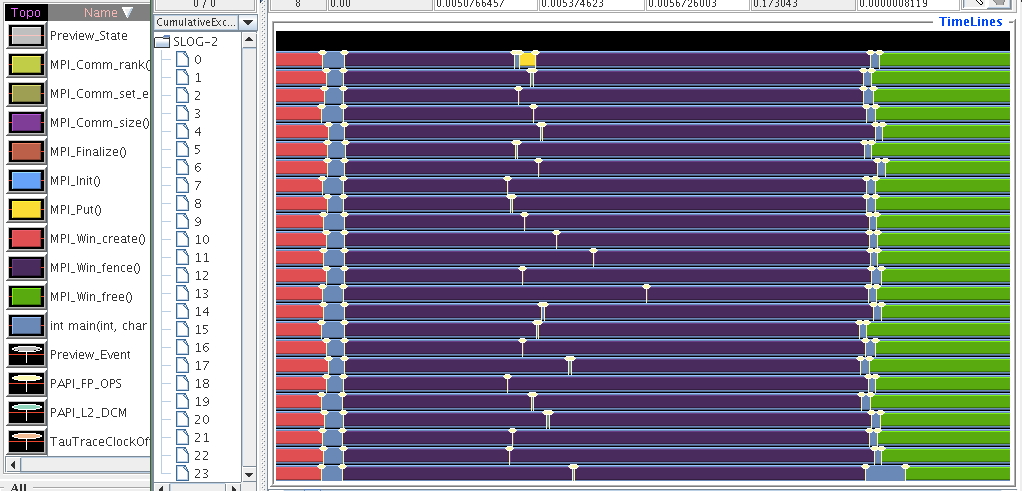
\includegraphics[scale=.4]{lonestar-twonode-put}%putblock
  \caption{A trace of a one-sided communication epoch where process zero only originates
  a one-sided transfer}
  \label{fig:putblock}
\end{figure}

As a further restriction, you can not mix \indexmpishow{MPI_Get} with \indexmpishow{MPI_Put}
or \indexmpishow{MPI_Accumulate} calls in a single epoch. Hence, we can
characterize an epoch as an \indextermsub{access}{epoch} on the
origin, and as an \indextermsub{exposure}{epoch} on the target.

\Level 1 {Fence assertions}

You can give various hints to the system about this epoch versus the ones
before and after through the \n{assert} parameter.
\begin{itemize}
\item \indexmpidef{MPI_MODE_NOSTORE}
  This value can be specified or not per process.
\item \indexmpidef{MPI_MODE_NOPUT}
  This value can be specified or not per process.
\item \indexmpidef{MPI_MODE_NOPRECEDE}
  This value has to be specified or not the same on all processes.
\item \indexmpidef{MPI_MODE_NOSUCCEED}
  This value has to be specified or not the same on all processes.
\end{itemize}

Example:
\begin{lstlisting}
MPI_Win_fence((MPI_MODE_NOPUT | MPI_MODE_NOPRECEDE), win);
MPI_Get( /* operands */, win);
MPI_Win_fence(MPI_MODE_NOSUCCEED, win);
\end{lstlisting}

Assertions are an integer parameter: you can combine assertions by
adding them or using logical-or.
The value zero is always correct. For further information, see
section~\ref{sec:mpi-assert}.

\Level 1 {Non-global target synchronization}
\label{sec:ref:post-wait}

The `fence' mechanism (section~\ref{sec:fence}) uses a global synchronization on the
communicator of the window, giving a program a \ac{BSP} like character.
As such it is good for applications where
the processes are largely synchronized, but it may 
lead to performance inefficiencies if processors are not in step which each other. 
Also, global synchronization may have hardware support, making this less
restrictive than it may at first seem.

There is a mechanism that is more fine-grained, by using synchronization only 
on a processor \indexterm{group}. This takes four different calls, two for starting
and two for ending the epoch, separately for target and origin.
\begin{figure}[ht]
  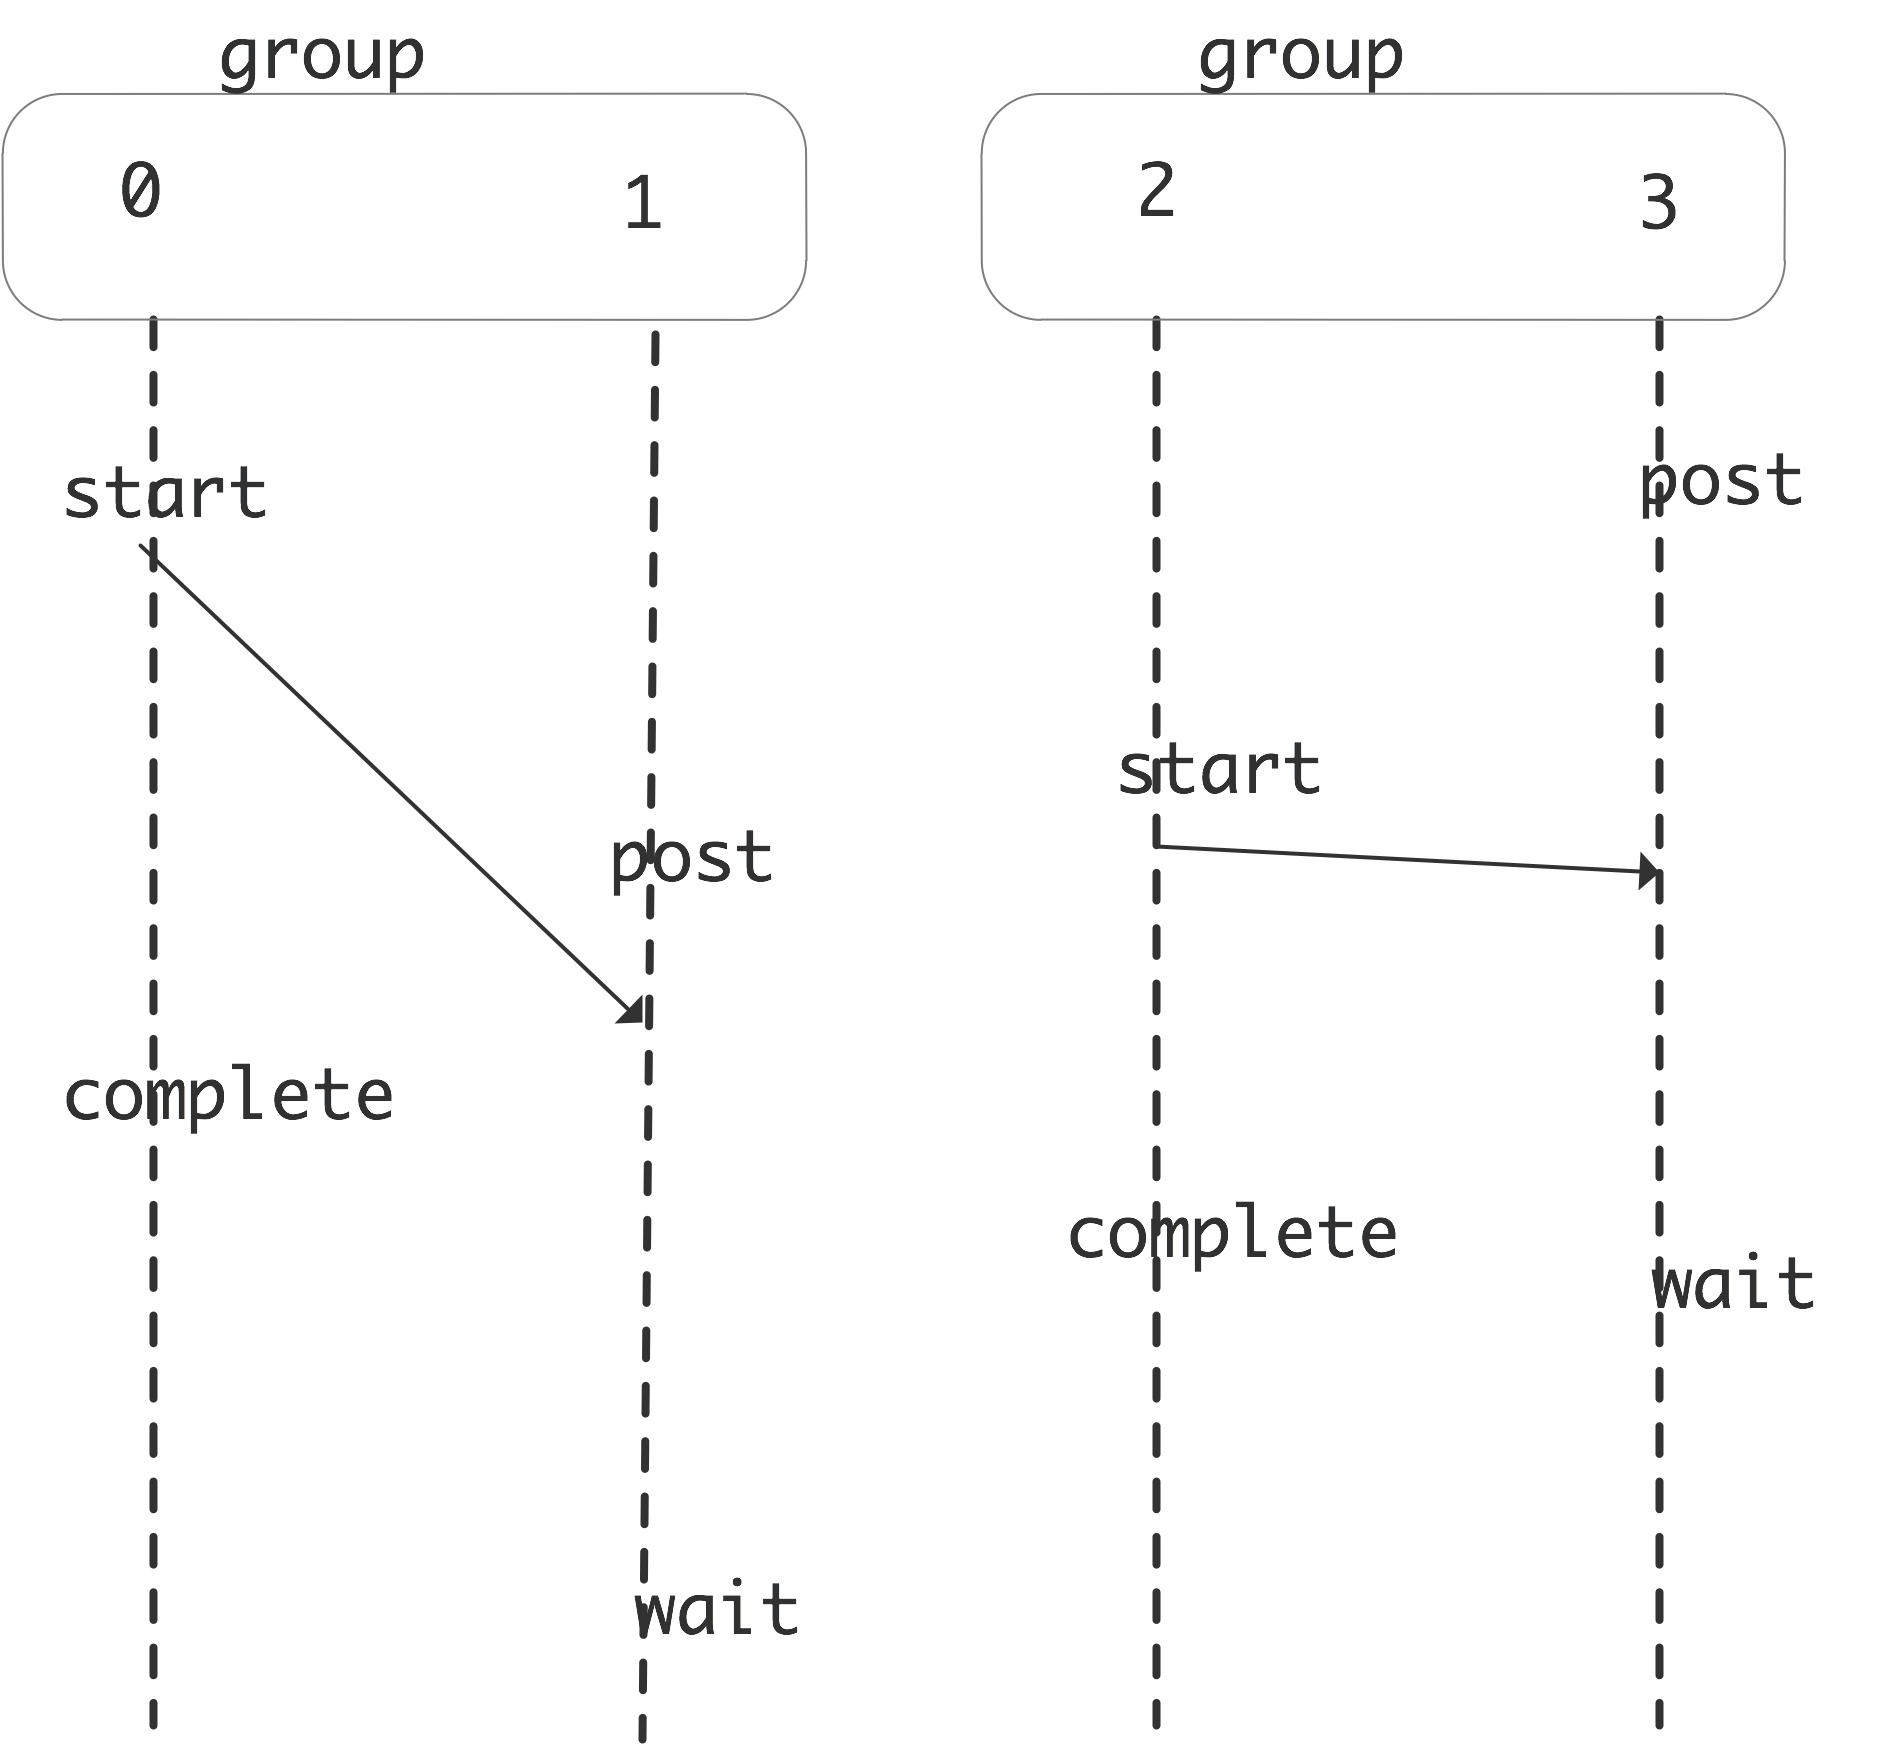
\includegraphics[scale=.1]{postwait}
  \caption{Window locking calls in fine-grained active target synchronization}
  \label{fig:postwait}
\end{figure}

You start and complete an \indextermsub{exposure}{epoch} with
\indexmpishow{MPI_Win_post}~/ \indexmpishow{MPI_Win_wait}:
\begin{lstlisting}
int MPI_Win_post(MPI_Group group, int assert, MPI_Win win)
int MPI_Win_wait(MPI_Win win)
\end{lstlisting}
In other words, this turns your window into the \indexterm{target} for a remote access.
There is a non-blocking version \indexmpidef{MPI_Win_test}
of \indexmpidef{MPI_Win_wait}.

You start and complete an \indextermsub{access}{epoch} with
\indexmpidef{MPI_Win_start}~/ \indexmpidef{MPI_Win_complete}:
\begin{lstlisting}
int MPI_Win_start(MPI_Group group, int assert, MPI_Win win)
int MPI_Win_complete(MPI_Win win)
\end{lstlisting}
In other words, these calls border the access to a remote window, with the current processor
being the \indexterm{origin} of the remote access.

In the following snippet a single processor puts data on one
other. Note that they both have their own definition of the group, and
that the receiving process only does the post and wait calls.
%
\cverbatimsnippet[examples/mpi/c/postwaitwin.c]{postwaittwo}

Both pairs of operations declare a
\indextermbus{group of}{processors}; see section~\ref{sec:comm-group}
for how to get such a group from a communicator.
On an origin processor you would specify a group that includes the targets
you will interact with, on a target processor you specify a group
that includes the possible origins.

\Level 0 {Put, get, accumulate}
\label{sec:putget}

We will now look at the first three routines for doing one-sided
operations: the Put, Get, and Accumulate call. (We will look at
so-called `atomic' operations in section~\ref{sec:mpi-atomic}.)
These calls are somewhat
similar to a Send, Receive and Reduce, except that of course only one
process makes a call.
Since one process does all the work, its calling sequence contains
both a description of the data on the origin (the calling process) and
the target (the affected other process).

As in the two-sided case, \indexmpishow{MPI_PROC_NULL} can be used as
a target rank.

The Accumulate routine has an \indexmpishow{MPI_Op}
argument that can be any of the usual operators, but no
user-defined ones (see section~\ref{sec:operator-list}).

\Level 1 {Put}
\label{sec:mpi-put}

The \indexmpiref{MPI_Put} call can be considered as a one-sided
send. As such, it needs to specify
\begin{itemize}
\item the target rank
\item the data to be sent from the origin, and
\item the location where it is to be written on the target.
\end{itemize}

The description of the data on the origin is the usual trio of
buffer/count/datatype. However, the description of the data on the
target is more complicated. It has a count and a datatype, but additionally
it has a
\emph{displacement}\index{window!displacement} with respect to the
start of the window on the target. This displacement can be given in
bytes, so its type is \indexmpishow{MPI_Aint}, but strictly speaking
it is a multiple of the displacement unit that was specified in the
window definition.

Specifically, data is written starting at
\[ \mathtt{window\_base} + \mathtt{target\_disp}\times \mathtt{disp\_unit}. \]


\includegraphics[scale=.4]{windowdisp}

Here is a single put operation. Note that the window create and window fence calls
are collective, so they have to be performed on all processors
of the communicator that was used in the create call.
%
\cverbatimsnippet[examples/mpi/c/putfence.c]{putfence}

\begin{fortrannote}{Displacement unit}
  The \n{disp_unit} variable is declared as an integer of `kind'
  \indexmpishow{MPI_ADDRESS_KIND}:
\fverbatimsnippet[examples/mpi/f08/putfence.F90]{fdisplacementtype}

Prior to \fstandard{2008},
specifying a literal constant, such as~\n{0}, could lead to bizarre
runtime errors; the solution was to specify a zero-valued variable
of the right type.
With the \indextermtt{mpi_f08} module this
is no longer allowed. Instead you get an error such as
\begin{verbatim}
error #6285: There is no matching specific subroutine for this generic subroutine call.   [MPI_PUT]
\end{verbatim}
\end{fortrannote}

\begin{pythonnote}{MPI one-sided transfer routines}
  \indexmpishow{MPI_Put} (and Get and Accumulate)
    accept at minimum the origin buffer and the target rank.
    The displacement is by default zero.
\end{pythonnote}

\begin{exercise}
  \label{ex:rightput}
  Revisit exercise~\ref{ex:serialsend} and solve it using
  \indexmpishow{MPI_Put}.
  \skeleton{rightput}
\end{exercise}

\begin{exercise}
  \label{ex:randomput}
  Write code where:
  \begin{itemize}
  \item
    process~0 computes a random number~$r$
  \item if $r<.5$, zero writes in the window on~1;
  \item if $r\geq .5$, zero writes in the window on~2.
  \end{itemize}
  \skeleton{randomput}
\end{exercise}

\Level 1 {Get}

The \indexmpiref{MPI_Get} call is very similar.

Example:
%
\cverbatimsnippet[examples/mpi/c/getfence.c]{getfence}
%
We make a null window on processes that do not participate.
%
\pverbatimsnippet[examples/mpi/p/getfence.py]{getfencep}

\Level 1 {Put and get example: halo update}

\begin{wrapfigure}{r}{3in}
  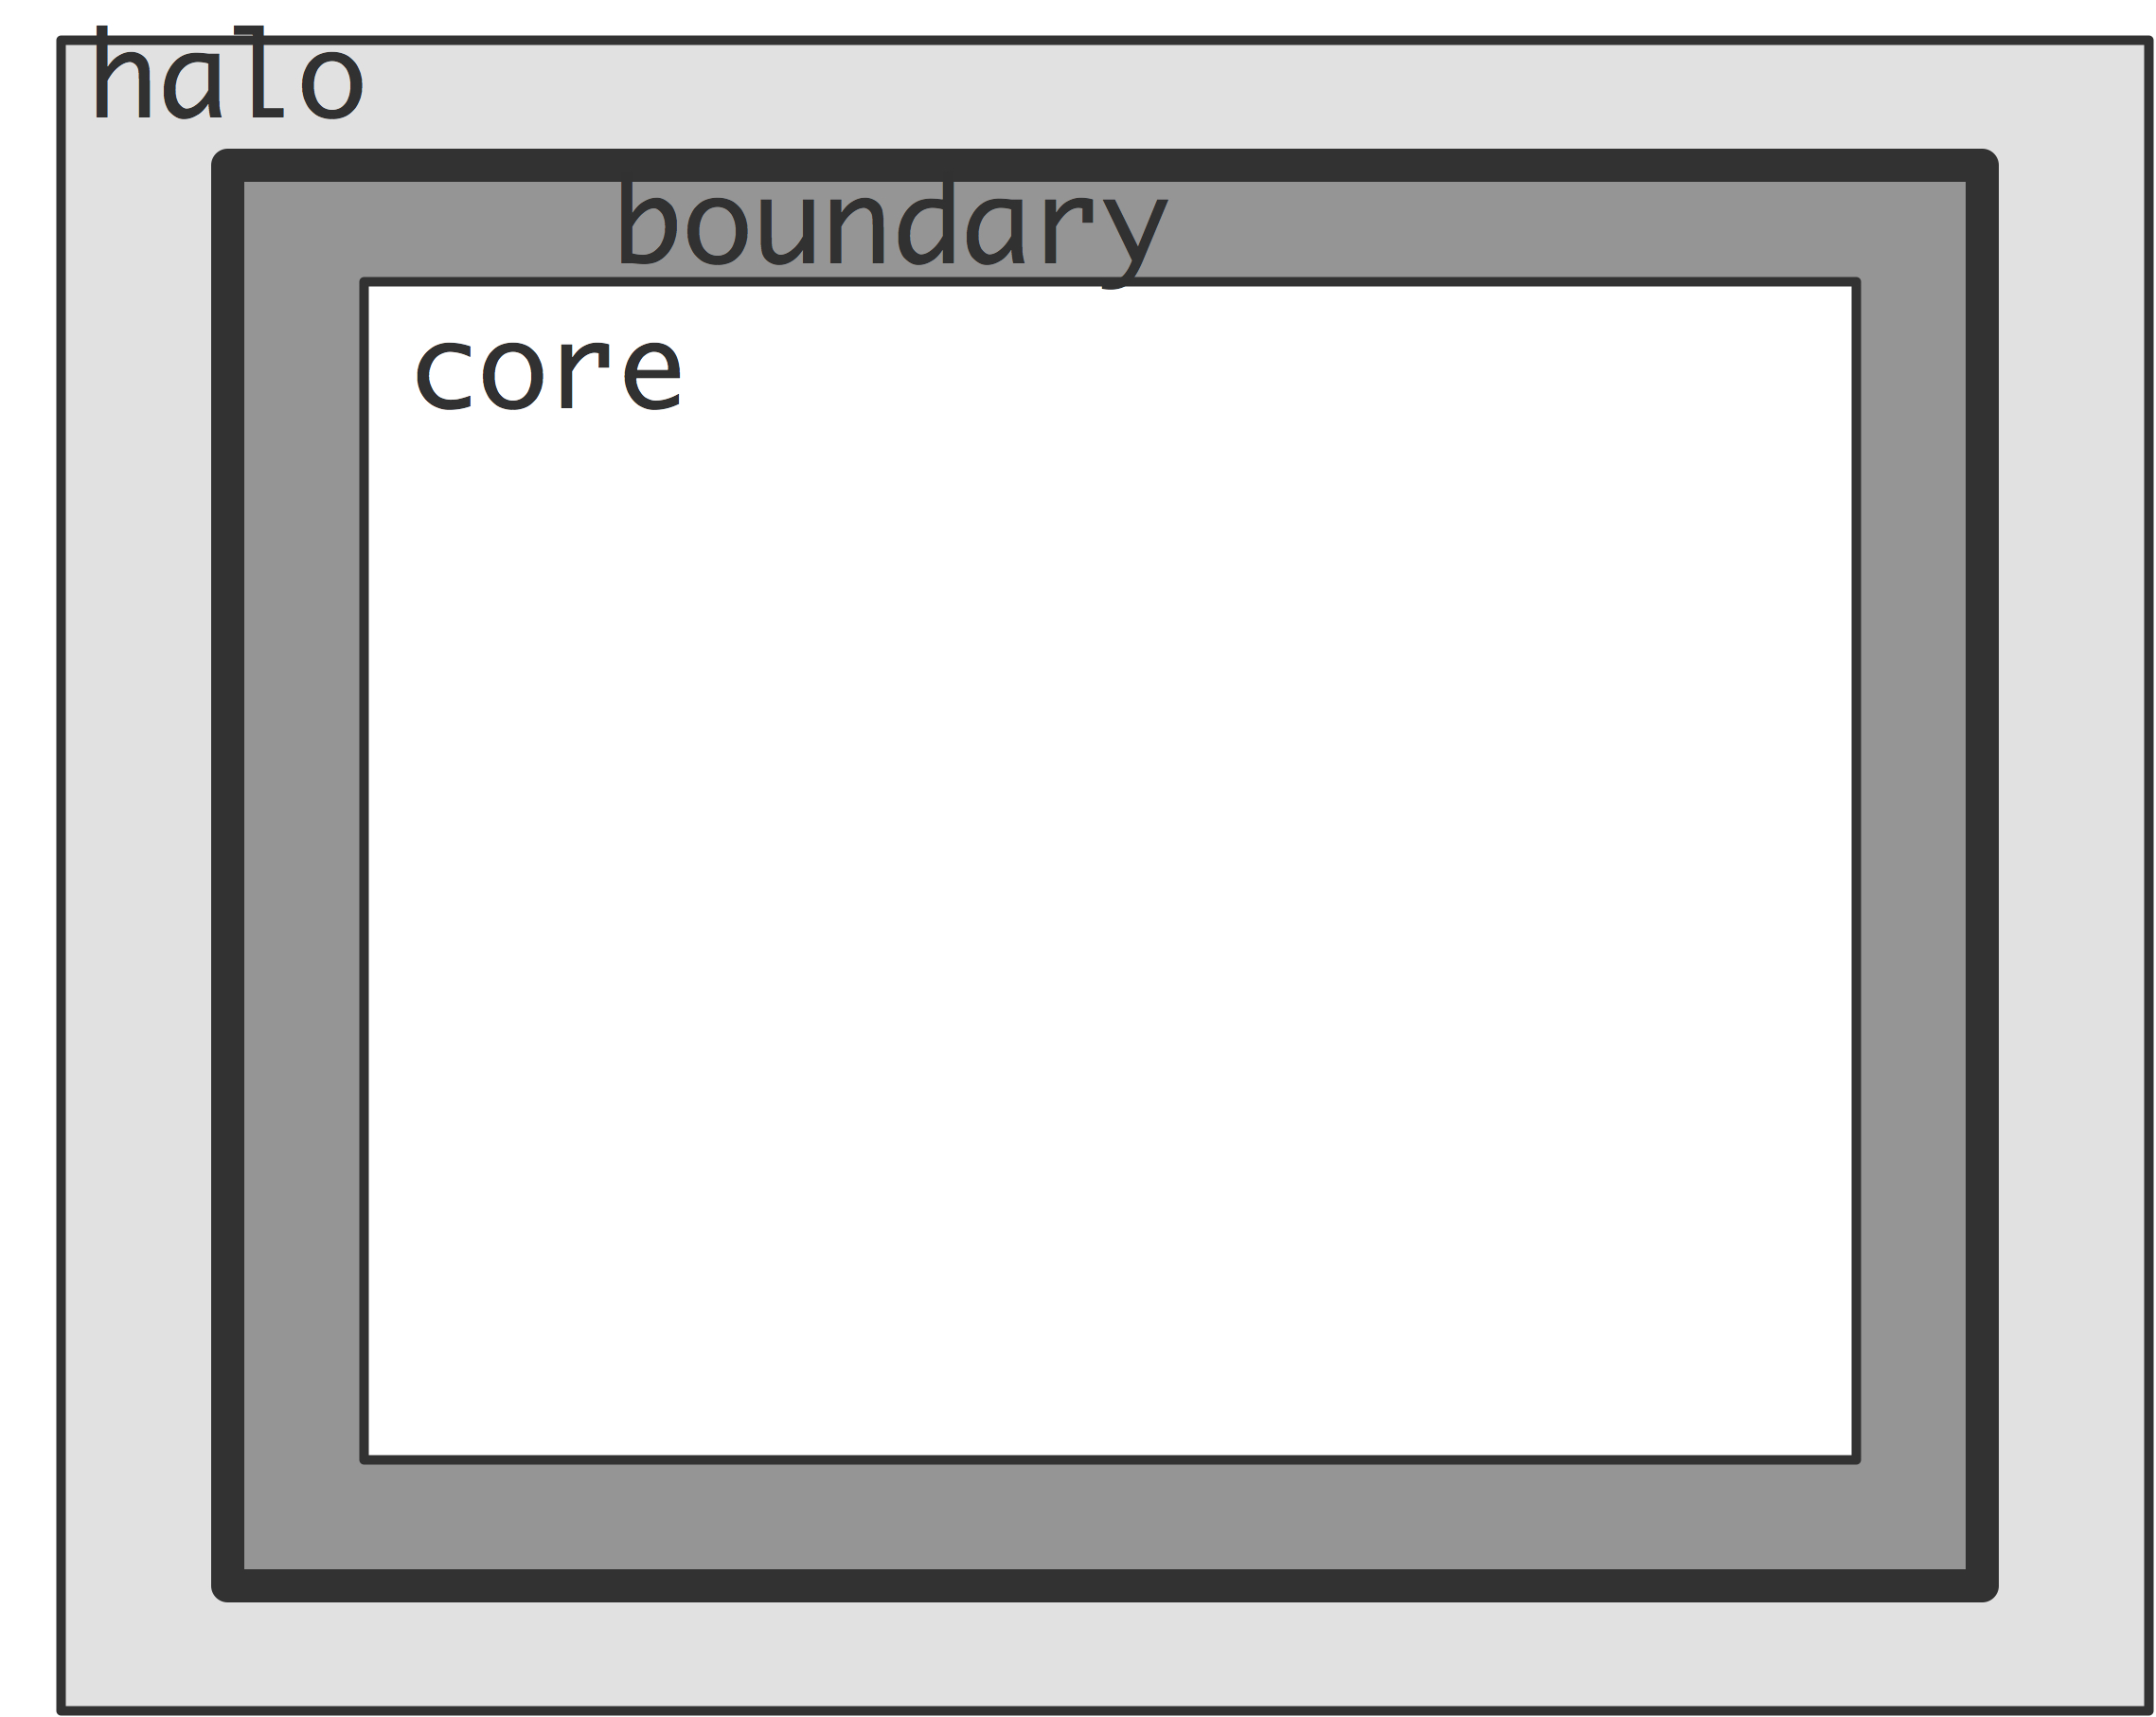
\includegraphics[scale=.08]{core-update}
\end{wrapfigure}
%
As an example, let's look at \indextermbus{halo}{update}.
The array~\n{A} is updated using the local values and the halo
that comes from bordering processors, either through Put or Get operations.

In a first version we separate computation and communication.
Each iteration has two fences. Between the two fences in the loop body
we do the \indexmpishow{MPI_Put} operation; between the second and and first one
of the next iteration there is only computation, so we add the
\indexmpishow{MPI_MODE_NOPRECEDE} and \indexmpishow{MPI_MODE_NOSUCCEED} assertions. 
The \indexmpishow{MPI_MODE_NOSTORE} assertion
states that the local window was not updated: the Put operation only
works on remote windows.
\begin{lstlisting}
for ( .... ) {
  update(A); 
  MPI_Win_fence(MPI_MODE_NOPRECEDE, win); 
  for(i=0; i < toneighbors; i++) 
    MPI_Put( ... );
  MPI_Win_fence((MPI_MODE_NOSTORE | MPI_MODE_NOSUCCEED), win); 
  }
\end{lstlisting}
For much more about
assertions, see section~\ref{sec:mpi-assert} below.

Next, we split the update in the core part, which can be done purely
from local values, and the boundary, which needs local and halo
values. Update of the core can overlap the communication of the halo.
\begin{lstlisting}
for ( .... ) {
  update_boundary(A); 
  MPI_Win_fence((MPI_MODE_NOPUT | MPI_MODE_NOPRECEDE), win); 
  for(i=0; i < fromneighbors; i++) 
    MPI_Get( ... );
  update_core(A); 
  MPI_Win_fence(MPI_MODE_NOSUCCEED, win); 
  }
\end{lstlisting}
The \indexmpishow{MPI_MODE_NOPRECEDE} and \indexmpishow{MPI_MODE_NOSUCCEED}
 assertions still hold, but the
\n{Get} operation implies that instead of \indexmpishow{MPI_MODE_NOSTORE} in the
second fence, we use \indexmpishow{MPI_MODE_NOPUT} in the first.

\Level 1 {Accumulate}

A~third one-sided routine
is \indexmpiref{MPI_Accumulate} which does a reduction operation on the results
that are being put.

Accumulate is an atomic reduction with remote result.
This means that multiple accumulates to a single target
in the same epoch give the correct result.
As with \indexmpishow{MPI_Reduce}, the 
order in which the operands are accumulated is undefined.

The same predefined operators are available, but no
user-defined ones. There is one extra operator: \indexmpidef{MPI_REPLACE},
this has the effect that only the last result to arrive is retained.

\begin{exercise}
  Implement an `all-gather' operation using one-sided communication:
  each processor stores a single number, and you want each processor
  to build up an array that contains the values from all
  processors. Note that you do not need a special case for a processor
  collecting its own value: doing `communication' between a processor
  and itself is perfectly legal.
\end{exercise}

\begin{figure}[ht]
  \includegraphics[scale=.5]{workpool}
  \caption{Pool of work descriptors with shared stack pointers}
  \label{fig:workpool}
\end{figure}

For the next exercise, refer to figure~\ref{fig:workpool}.

\begin{exercise}
  \label{ex:countdown}

  Implement a shared counter:
  \begin{itemize}
  \item One process maintains a counter;
  \item Iterate: all others at random moments update this counter.
  \item When the counter is no longer positive, everyone stops iterating.
  \end{itemize}
  The problem here is data synchronization: does everyone see the
  counter the same way?
\end{exercise}

\Level 1 {Ordering and coherence of RMA operations}

There are few guarantees about what happens inside one epoch.
\begin{itemize}
\item No ordering of Get and Put/Accumulate operations: if you do
  both, there is no guarantee whether the Get will find the value
  before or after the update.
\item No ordering of multiple Puts. It is safer to do an Accumulate.
\end{itemize}
The following operations are well-defined inside one epoch:
\begin{itemize}
\item Instead of multiple Put operations, use Accumulate with
  \indexmpishow{MPI_REPLACE}.
\item \indexmpishow{MPI_Get_accumulate} with
  \indexmpishow{MPI_NO_OP} is safe.
\item Multiple Accumulate operations from one origin are done in
  program order by default. To allow reordering, for instance to have
  all reads happen after all writes, use the info parameter
  when the window is created; section~\ref{sec:window-info}.
\end{itemize}

\Level 1 {Request-based operations}

Analogous to \indexmpishow{MPI_Isend} there are request-based one-sided operations:
%
\indexmpiref{MPI_Rput}
%
and similarly \indexmpishow{MPI_Rget} and
\indexmpishow{MPI_Raccumulate}
and \indexmpishow{MPI_Rget_accumulate}.
These only apply to passive target synchronization.
Any \indexmpishow{MPI_Win_flush...} call also terminates these transfers.

\Level 1 {Atomic operations}
\label{sec:mpi-atomic}
\index{atomic operation!MPI|(}

One-sided calls are said to emulate shared memory in MPI, but 
the put and get calls are not enough for certain scenarios with shared
data. Consider the scenario where:

\begin{itemize}
\item One process stores a table of work descriptors, and a pointer to
  the first unprocessed descriptor;
\item Each process reads the pointer, reads the corresponding
  descriptor, and increments the pointer; and
\item A process that has read a descriptor then executes the
  corresponding task.
\end{itemize}

The problem is that reading and updating the pointer is not an
\emph{atomic operation}, so
it is possible that multiple processes get hold of the same value;
conversely, multiple updates of the pointer may lead to work
descriptors being skipped.
These different overall behaviors, depending on precise timing of lower level events,
are called a \indexterm{race condition}.

In \mpistandard{3} some atomic routines have been added.
Both \indexmpiref{MPI_Fetch_and_op} and \indexmpiref{MPI_Get_accumulate}
atomically retrieve data from the window indicated,
and apply an operator, combining the data on the target
with the data on the origin.
Unlike Put and Get, it is safe to have multiple atomic operations
in the same epoch.

Both routines perform the same operations: return data before the
operation, then atomically update data on the target, but
\indexmpishow{MPI_Get_accumulate} is more flexible in data type
handling. The more simple routine, \indexmpishow{MPI_Fetch_and_op},
which operates on only a single element,
allows for faster implementations, in particular through hardware support.

Use of \indexmpishow{MPI_NO_OP} as the \indexmpishow{MPI_Op}
turns these routines into an atomic Get. Similarly, using
\indexmpishow{MPI_REPLACE} turns them into an atomic Put.

\begin{exercise}
  \label{ex:countdownop}
  Redo exercise~\ref{ex:countdown} using \indexmpishow{MPI_Fetch_and_op}. The
  problem is again to make sure all processes have the same view of
  the shared counter.

  Does it work to make the fetch-and-op conditional? Is there a way to
  do it unconditionally? What should the `break' test be, seeing that
  multiple processes can update the counter at the same time?
\end{exercise}

\begin{example}
  A root process has a table of data; the other processes do 
  atomic gets and update of that data using
  \indexterm{passive target synchronization} through \indexmpishow{MPI_Win_lock}.
  %
  \cverbatimsnippet[examples/mpi/c/fetchop.c]{fetchop}
  %
  \pverbatimsnippet[examples/mpi/p/passive.py]{fetchopp}
\end{example}

Finally, \indexmpiref{MPI_Compare_and_swap} swaps the origin and
target data if the target data equals some comparison value.

\Level 2 {A case study in atomic operations}

Let us consider an example where a process,
identified by \lstinline+counter_process+,
has a table of work descriptors,
and all processes, including the counter process,
take items from it to work on.
To avoid duplicate work, the counter process has as counter
that indicates the highest numbered available item.
The part of this application that we simulate is this:
\begin{enumerate}
\item a process reads the counter, to find an available work item; and
\item subsequently decrements the counter by one.
\end{enumerate}

We initialize the window content, under the separate memory model:
%
\cverbatimsnippet[examples/mpi/c/countdownop.c]{countdowninitput}

We start by considering the naive approach, where we execute the above scheme
literally with \indexmpishow{MPI_Get} and \indexmpishow{MPI_Put}:
%
\cverbatimsnippet[examples/mpi/c/countdownput.c]{countdowngetput}

This scheme is correct if only process
has a true value for \lstinline+i_am_available+:
that processes `owns' the current counter values,
and it correctly updates the counter
through the \indexmpishow{MPI_Put} operation.
However, if more than one process is available,
they get duplicate counter values, and the update
is also incorrect.
If we run this program, we see that the counter did not get
decremented by the total number of `put' calls.

\begin{exercise}
  Supposing only one process is available, what is the function
  of the middle of the three fences? Can it be omitted?
\end{exercise}

We can fix the decrement of the counter by using \indexmpishow{MPI_Accumulate}
for the counter update, since it is atomic:
multiple updates in the same epoch all get processed.
%
\cverbatimsnippet[examples/mpi/c/countdownacc.c]{countdowngetacc}

This scheme still suffers from the problem that processes will obtain duplicate
counter values. The true solution is to combine the `get' and `put' operations
into one atomic action; in this case \indexmpishow{MPI_Fetch_and_op}:
%
\cverbatimsnippet[examples/mpi/c/countdownop.c]{fetchopfence}

Now, if there are multiple accesses, each retrieves the counter value
and updates it in one atomic, that is, indivisible, action.

\index{atomic operation!MPI|)}

\Level 0 {Passive target synchronization}
\label{sec:passive-sync}

In \indexterm{passive target synchronization} only the origin is
actively involved: the target makes no synchronization calls.
This means that the origin process remotely locks the window
on the target, performs a one-sided transfer, and releases the window
by unlocking it again.

During an access epoch, also called an
\indextermsubdef{passive target}{epoch} in this case
(the concept of `exposure epoch' makes no sense with passive target synchronization),
a~process can initiate and finish a one-sided
transfer. Typically it will lock the window with
\indexmpiref{MPI_Win_lock}:

\begin{lstlisting}
if (rank == 0) {
  MPI_Win_lock (MPI_LOCK_EXCLUSIVE, 1, 0, win);
  MPI_Put (outbuf, n, MPI_INT, 1, 0, n, MPI_INT, win);
  MPI_Win_unlock (1, win);
}
\end{lstlisting}

\begin{remark}
  The possibility to lock a window is not guaranteed for windows
  that are not created (possibly internally) by \indexmpishow{MPI_Alloc_mem},
  that is, all but \indexmpishow{MPI_Win_create}.
\end{remark}

\Level 1 {Lock types}

A lock is needed to start an \indextermsub{access}{epoch}, that is,
for an origin to acquire the capability to access a target.
You can either acquire a lock on a specific process with \indexmpishow{MPI_Win_lock},
or on all processes (in a communicator) with \indexmpishow{MPI_Win_lock_all}.
Unlike \indexmpishow{MPI_Win_fence}, this is not a collective call.
Also, it is possible to have multiple access epochs through \indexmpishow{MPI_Win_lock}
active simultaenously.

The two lock types are:
\begin{itemize}
\item \indexmpishow{MPI_LOCK_SHARED}: multiple processes can access 
  the window on the same rank.
  If multiple processes perform a \indexmpishow{MPI_Get} call there
  is no problem; with \indexmpishow{MPI_Put} and similar calls
  there is a consistency problem; see below.
\item \indexmpishow{MPI_LOCK_EXCLUSIVE}: an origin gets exclusive access to the
  window on a certain target.
  Unlike the shared lock, this has no consistency problems.
\end{itemize}

You can only specify a lock type in \indexmpishow{MPI_Win_lock};
\indexmpishow{MPI_Win_lock_all} is always shared.

To unlock a window, use
\indexmpiref{MPI_Win_unlock}, % includes unlock_all
respectively \indexmpidef{MPI_Win_unlock_all}.

\begin{exercise}
  \label{ex:lockandfetch}
  Investigate atomic updates using passive target synchronization.
  Use \indexmpishow{MPI_Win_lock} with an exclusive lock, which
  means that each process only acquires the lock when it absolutely has to.
  \begin{itemize}
  \item All processs but one update a window:
\begin{lstlisting}
int one=1;
MPI_Fetch_and_op(&one, &readout,
    MPI_INT, repo, zero_disp, MPI_SUM,
    the_win);
\end{lstlisting}
  \item while the remaining process spins until the others have performed their update.
  \end{itemize}
  Use an atomic operation for the latter process to read out the shared value.\\
  Can you replace the exclusive lock with a shared one?
  \skeleton{lockfetch}
\end{exercise}

\begin{exercise}
  \label{ex:lockfetchshared}
  As exercise~\ref{ex:lockandfetch}, but now use a shared lock:
  all processes acquire the lock simultaneously and keep it as long as is needed.

  The problem here is that coherence between window buffers and local variables is
  now not forced by a fence or releasing a lock. Use \lstinline{MPI_Win_flush_local} to
  force coherence of a window (on another process) and the local variable from
  \lstinline{MPI_Fetch_and_op}.
  \skeleton{lockfetchshared}
\end{exercise}

\Level 1 {Lock all}
\label{sec:win-lock-all}

To lock the windows of all processes in the group of the windows, use
\indexmpiref{MPI_Win_lock_all}. This is not a collective call:
the `all' part refers to the fact that one process is locking the
window on all processes.
\begin{itemize}
\item
  The assertion value can be zero, or \indexmpidef{MPI_MODE_NOCHECK},
  which asserts that no other process will acquire a competing lock.
\item There is no `locktype' parameter: this is a shared lock.
\end{itemize}

The corresponding unlock is
\indexmpishow{MPI_Win_unlock_all}.

The expected use of a `lock/unlock all' is that they surround
an extended epoch with get/put and flush calls.

\Level 1 {Completion and consistency in passive target synchronization}

In one-sided transfer one should keep straight the multiple instances
of the data, and the various \indextermdef{completion}s that effect
their \emph{consistency}\index{window!consistency}.
\begin{itemize}
\item The user data. This is the buffer that is passed to an RMA call.
  For instance, after an \indexmpishow{MPI_Put} call, but still in an
  access epoch, the user buffer is not safe to reuse. Making sure the
  buffer has been transferred is called \indextermsub{local}{completion}.
\item The window data. While this may be publicly accessible, it is
  not necessarily always consistent with internal copies.
\item The remote data. Even a successful \indexmpishow{MPI_Put} does not guarantee
  that the other process has received the data. A~successful transfer
  is a \indextermsub{remote}{completion}.
\end{itemize}

As observed, \ac{RMA} operations are nonblocking, so we need
mechanisms to ensure that an operation is completed,
and to ensure \emph{consistency}\index{window!consistency} of the
user and window data.

Completion of the \ac{RMA} operations in a  passive target epoch
is ensured with
\indexmpishow{MPI_Win_unlock} or \indexmpishow{MPI_Win_unlock_all},
similar to the use of \indexmpishow{MPI_Win_fence}
in active target synchronization.

If the passive target epoch is of greater duration,
and no unlock operation is used to ensure completion,
the following calls are available.

\begin{remark}
  Using flush routines with active target synchronization
  (or generally outside a passive target epoch) you are
  likely to get a message
\begin{verbatim}
Wrong synchronization of RMA calls
\end{verbatim}
\end{remark}

\Level 2 {Local completion}

The call \indexmpiref{MPI_Win_flush_local} 
ensure that all operations with a given target is completed at the origin.
For instance, for calls to \indexmpishow{MPI_Get} or
\indexmpishow{MPI_Fetch_and_op} the local result is available after
the \indexmpishow{MPI_Win_flush_local}.

With \indexmpishow{MPI_Win_flush_local_all} local operations are
concluded for all targets. This will typically be used
with \indexmpishow{MPI_Win_lock_all} (section~\ref{sec:win-lock-all}).

\Level 2 {Remote completion}

The calls
\indexmpiref{MPI_Win_flush} and
\indexmpishow{MPI_Win_flush_all}
effect completion of all outstanding \ac{RMA} operations
on the target, so that
other processes can access its data.
This is useful for \indexmpishow{MPI_Put} operations,
but can also be used for atomic operations
such as \indexmpishow{MPI_Fetch_and_op}.

\Level 2 {Window synchronization}

Under the
\emph{separate memory model}\index{window!memory!separate},
the user code can hold a buffer that is not coherent with the internal
window data. The call \indexmpidef{MPI_Win_sync} synchronizes
private and public copies of the window.

\Level 0 {More about window memory}

\Level 1 {Memory models}
\label{sec:win-model}

You may think that the window memory is the same as the buffer you
pass to \indexmpishow{MPI_Win_create} or that you get from
\indexmpishow{MPI_Win_allocate} (section~\ref{sec:win-alloc}).
This is not necessarily true, and the
actual state of affairs is called the
\emph{memory model}\index{window!memory!model}%
\index{memory!model|see{window, memory, model}}.
There are two memory models:
\index{window!memory|seealso{memory model}}%pyskip
\begin{itemize}
\item Under the \emph{unified}\index{window!memory!model!unified} memory
  model, the buffer in process space is indeed the window memory,
  or at least they are kept \emph{coherent}\index{memory!coherent}.
  This
  means that after \emph{completion}\index{epoch!completion} of an
  epoch you can read the window contents from the buffer.
  To get this, the window needs to be created with
  \indexmpishow{MPI_Win_allocate_shared}.
  This memory model is required for MPI shared memory; chapter~\ref{ch:mpi-shared}.
\item Under the \emph{separate}\index{window!memory!model!separate} memory
  model, the buffer in process space is the
  \indextermsub{private}{window} and the target of put/get operations
  is the \indextermsub{public}{window} and the two are not the same
  and are not kept coherent. Under this model, you need to do an
  explicit get to read the window contents.
\end{itemize}

You can query the model of a window
using the \indexmpidef{MPI_Win_get_attr} call
with the \indexmpidef{MPI_WIN_MODEL} keyword:
%
\cverbatimsnippet{winmodel}
%
with possible values:
\begin{itemize}
\item \indexmpishow{MPI_WIN_SEPARATE},
\item \indexmpishow{MPI_WIN_UNIFIED},
\end{itemize}
For more on attributes, see section~\ref{sec:win-attr}.

\Level 1 {Dynamically attached memory}
\label{sec:win-dynamic}

In section~\ref{sec:win-alloc} we looked at simple ways to create a
window and its memory.

It is also possible to have windows where the size is dynamically set.
Create a dynamic window with
\indexmpiref{MPI_Win_create_dynamic}
and attach
memory to the window with
%
\indexmpiref{MPI_Win_attach}.

At first sight, the code looks like splitting up a \indexmpishow{MPI_Win_create}
call into separate creation of the window and declaration of the buffer:
%
\cverbatimsnippet[examples/mpi/c/windynamic.c]{winattach}
(where the \lstinline{window_buffer} represents memory that has been allocated.)

However, there is an important difference in how the window is addressed
in \ac{RMA} operations.
With all other window models, the displacement parameter is measured relative
in units from the start of the buffer, here the displacement
is an absolute address. This means that we need to get the address
of the window buffer with \indexmpishow{MPI_Get_address} and
communicate it to the other processes:
%
\cverbatimsnippet[examples/mpi/c/windynamic.c]{addrbcast}

Location of the data, that is, the displacement parameter,
is then given as an absolute location
of the start of the buffer plus a count in bytes;
in other words, the \indexterm{displacement unit} is~1.
In this example we use \indexmpishow{MPI_Get} to find the second
integer in a window buffer:
%
\cverbatimsnippet[examples/mpi/c/windynamic.c]{windynamicget}

Notes.
\begin{itemize}
\item 
  The attached memory can be released with
  %
  \indexmpiref{MPI_Win_detach}.
\item The above fragments show that an origin process has the actual
  address of the window buffer. It is an error to use this if the
  buffer is not attached to a window.
\item In particular, one has to make sure that the attach call is
  concluded before performing \ac{RMA} operations on the window.
\end{itemize}

\Level 1 {Window usage hints}
\label{sec:window-info}

The following keys can be passed as info argument:
\begin{itemize}
\item \indexmpishow{no_locks}: if set to true, passive target synchronization
  (section~\ref{sec:passive-sync}) will not be used on this window.
\item \indexmpishow{accumulate_ordering}: a comma-separated list of
  the keywords \indextermtt{rar}, \indextermtt{raw},
  \indextermtt{war}, \indextermtt{waw} can be specified. This
  indicates that reads or writes from \indexmpishow{MPI_Accumulate} or
  \indexmpishow{MPI_Get_accumulate} can be reordered, subject to
  certain constraints.
\item \indexmpishow{accumulate_ops}: the value \indexmpishow{same_op}
  indicates that concurrent Accumulate calls use the same operator;
  \indexmpishow{same_op_no_op} indicates the same operator or
  \indexmpishow{MPI_NO_OP}.
\end{itemize}

\Level 1 {Window information}
\label{sec:win-attr}

The \indexmpishow{MPI_Info} parameter
(see section~\ref{sec:mpi-info} for info objects)
can be used to pass implementation-dependent 
information.

A number of attributes are stored with a window when it is created.
\begin{itemize}
\item \indexmpishow{MPI_WIN_BASE} for
  obtaining a pointer to the start of the window area:
\begin{lstlisting}
void *base;
MPI_Win_get_attr(win, MPI_WIN_BASE, &base, &flag)  
\end{lstlisting}
\item \indexmpishow{MPI_WIN_SIZE} and \indexmpishow{MPI_WIN_DISP_UNIT} for
  obtaining the size and \indextermbus{window}{displacement unit}:
\begin{lstlisting}
MPI_Aint *size;
MPI_Win_get_attr(win, MPI_WIN_SIZE, &size, &flag), 
int *disp_unit;
MPI_Win_get_attr(win, MPI_WIN_DISP_UNIT, &disp_unit, &flag), 
\end{lstlisting}
\item \indexmpishow{MPI_WIN_CREATE_FLAVOR} for determining
the type of create call used:
\begin{lstlisting}
int *create_kind;
MPI_Win_get_attr(win, MPI_WIN_CREATE_FLAVOR, &create_kind, &flag)
\end{lstlisting}
with possible values:
\begin{itemize}
\item \indexmpishow{MPI_WIN_FLAVOR_CREATE} if the window was create
  with \indexmpishow{MPI_Win_create};
\item \indexmpishow{MPI_WIN_FLAVOR_ALLOCATE} if the window was create
  with \indexmpishow{MPI_Win_allocate};
\item \indexmpishow{MPI_WIN_FLAVOR_DYNAMIC} if the window was create
  with \indexmpishow{MPI_Win_create_dynamic}. In this case the base is
  \indexmpishow{MPI_BOTTOM} and the size is zero;
\item \indexmpishow{MPI_WIN_FLAVOR_SHARED} if the window was create
  with \indexmpishow{MPI_Win_allocate_shared};
\end{itemize}
\item \indexmpishow{MPI_WIN_MODEL} for
  querying the window memory model; see section~\ref{sec:win-model}.
\end{itemize}

Get the group of processes (see section~\ref{sec:mpi-comm-group})
associated with a window:
\begin{lstlisting}
int MPI_Win_get_group(MPI_Win win, MPI_Group *group) 
\end{lstlisting}

Window information objects (see section~\ref{sec:mpi-info})
can be set and retrieved:
\begin{lstlisting}
int MPI_Win_set_info(MPI_Win win, MPI_Info info)
\end{lstlisting}
\begin{lstlisting}
int MPI_Win_get_info(MPI_Win win, MPI_Info *info_used)
\end{lstlisting}

\Level 0 {Assertions}
\label{sec:mpi-assert}

The routines
\begin{itemize}
\item (Active target synchronization)
  \indexmpishow{MPI_Win_fence},
  \indexmpishow{MPI_Win_post},
  \indexmpishow{MPI_Win_start};
\item (Passive target synchronization)
  \indexmpishow{MPI_Win_lock},
  \indexmpishow{MPI_Win_lockall},
\end{itemize}
take an argument
through which assertions can be passed about the activity before, after, and during the epoch.
The value zero is always allowed, by you can make your program more efficient by specifying
one or more of the following, combined by bitwise OR in C/C++ or
\n{IOR} in Fortran.

\begin{itemize}
\item \indexmpishow{MPI_Win_start} Supports the option:
  \begin{itemize}
    \item \indexmpishow{MPI_MODE_NOCHECK} the matching calls to \indexmpishow{MPI_Win_post} have already
    completed on all target processes when the call to \indexmpishow{MPI_Win_start} is
    made. The nocheck option can be specified in a start call if and
    only if it is specified in each matching post call. This is similar
    to the optimization of ``ready-send'' that may save a handshake when
    the handshake is implicit in the code. (However, ready-send is
    matched by a regular receive, whereas both start and post must
    specify the nocheck option.)
  \end{itemize}
\item \indexmpishow{MPI_Win_post} supports the following options:
  \begin{itemize}
  \item \indexmpishow{MPI_MODE_NOCHECK} the matching calls to \indexmpishow{MPI_Win_start} have not
    yet occurred on any origin processes when the call to \indexmpishow{MPI_Win_post}
    is made. The nocheck option can be specified by a post call if and
    only if it is specified by each matching start call.
  \item \indexmpishow{MPI_MODE_NOSTORE} the local window was not updated by local
    stores (or local get or receive calls) since last
    synchronization. This may avoid the need for cache synchronization
    at the post call.
  \item \indexmpishow{MPI_MODE_NOPUT} the local window will not be updated by put or
    accumulate calls after the post call, until the ensuing (wait)
    synchronization. This may avoid the need for cache synchronization
    at the wait call.
  \end{itemize}
\item \indexmpishow{MPI_Win_fence} supports the following options:
  \begin{itemize}
  \item \indexmpishow{MPI_MODE_NOSTORE} the local window was not updated by local
    stores (or local get or receive calls) since last synchronization.
  \item \indexmpishow{MPI_MODE_NOPUT} the local window will not be updated by put or
    accumulate calls after the fence call, until the ensuing (fence)
    synchronization.
  \item \indexmpishow{MPI_MODE_NOPRECEDE} the fence does not complete any sequence of
    locally issued RMA calls. If this assertion is given by any
    process in the window group, then it must be given by all
    processes in the group.
  \item \indexmpishow{MPI_MODE_NOSUCCEED} the fence does not start any
    sequence of locally issued RMA calls. If the assertion is given by
    any process in the window group, then it must be given by all
    processes in the group.
  \end{itemize}
\item \indexmpishow{MPI_Win_lock} and \indexmpishow{MPI_Win_lock_all}
  support the following option:
  \begin{itemize}
    \item \indexmpishow{MPI_MODE_NOCHECK} no other process holds, or will attempt to
    acquire a conflicting lock, while the caller holds the window
    lock. This is useful when mutual exclusion is achieved by other
    means, but the coherence operations that may be attached to the
    lock and unlock calls are still required.
  \end{itemize}
\end{itemize}

\Level 0 {Implementation}
\index{communication!one-sided, implementation of|(}

You may wonder how one-sided communication is realized\footnote{For
  more on this subject, see~\cite{thakur:ijhpca-sync}.}. Can a processor
somehow get at another processor's data? Unfortunately, no.

Active target synchronization is implemented in terms of two-sided communication.
Imagine that the first fence operation does nothing, unless it concludes prior
one-sided operations. The Put and Get calls do nothing involving communication,
except for marking with what processors they exchange data.
The concluding fence is where everything happens: first a global operation
determines which targets need to issue send or receive calls, then the
actual sends and receive are executed.

\begin{exercise}
  Assume that only Get operations are performed during an epoch. 
  Sketch how these are translated to send/receive pairs. 
  The problem here is how the senders find out that they need to send.
  Show that you can solve this with an \indexmpishow{MPI_Reduce_scatter} call.
\end{exercise}

The previous paragraph noted that a collective operation was necessary
to determine the two-sided traffic. Since collective operations induce
some amount of synchronization, you may want to limit this.

\begin{exercise}
  Argue that the mechanism with window post/wait/start/complete operations
  still needs a collective, but that this is less burdensome.
\end{exercise}

Passive target synchronization needs another mechanism entirely.  Here
the target process needs to have a background task (process, thread,
daemon,\ldots) running that listens for requests to lock the
window. This can potentially be expensive.

\index{communication!one-sided, implementation of|)}
\index{communication!one-sided|)}

\newpage
\Level 0 {Review questions}

Find all the errors in this code.
\begin{lstlisting}
#include <mpi.h>
#include <stdio.h>
#include <stdlib.h>

#define MASTER 0

int main(int argc, char *argv[])
{
  MPI_Init(&argc, &argv);
  MPI_Comm comm = MPI_COMM_WORLD;
  int r, p;
  MPI_Comm_rank(comm, &r);
  MPI_Comm_size(comm, &p);
  printf("Hello from %d\n", r);
  int result[1] = {0};
  //int assert = MPI_MODE_NOCHECK;
  int assert = 0;
  int one = 1;
  MPI_Win win_res;
  MPI_Win_allocate(1 * sizeof(MPI_INT), sizeof(MPI_INT), MPI_INFO_NULL, comm, &result[0], &win_res);
  MPI_Win_lock_all(assert, win_res);
  if (r == MASTER) {
    result[0] = 0;
    do{
      MPI_Fetch_and_op(&result, &result , MPI_INT, r, 0, MPI_NO_OP, win_res);  
      printf("result: %d\n", result[0]);
    } while(result[0] != 4);
    printf("Master is done!\n");
  } else {
    MPI_Fetch_and_op(&one, &result, MPI_INT, 0, 0, MPI_SUM, win_res);
  }
  MPI_Win_unlock_all(win_res);
  MPI_Win_free(&win_res);
  MPI_Finalize();
  return 0;
\end{lstlisting}
